% "{'classe':('PSI'),'chapitre':'cin_va','type':('application'),'titre':'Danse avec les robots', 'source':'ICNA 2017','comp':(''),'corrige':True}"
%\setchapterimage{fig_00.jpg}
\chapter*{Application \arabic{cptApplication} \\ 
Danse avec les robots -- \ifprof Corrigé \else Sujet \fi}
\addcontentsline{toc}{section}{Application \arabic{cptApplication} : Danse avec les robots -- \ifprof Corrigé \else Sujet \fi}

\iflivret \stepcounter{cptApplication} \else
\ifprof  \stepcounter{cptApplication} \else \fi
\fi

\setcounter{question}{0}
\marginnote{ICNA 2017.}
\marginnote[1cm]{
%\UPSTIcompetence[2]{B2-14}
%\UPSTIcompetence[2]{C1-05}
%\UPSTIcompetence[2]{C2-07}
}

\begin{marginfigure}
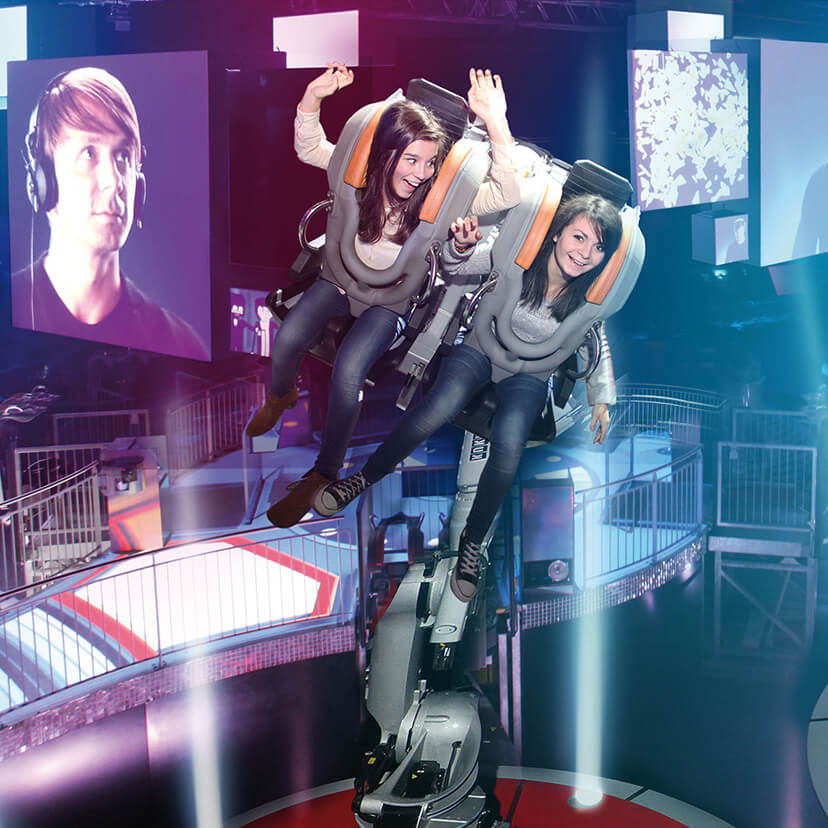
\includegraphics[width=\textwidth]{fig_01}
\end{marginfigure}



<< Danse avec les robots >> est une attraction du Futuroscope de Poitiers. Le principe consiste à attacher deux personnes au bout d'un bras de robot 5 axes. Les personnes sont ainsi remués au rythme de la musique.

On appelle nacelle l'ensemble de solides composé des sièges, des harnais de sécurité et des 2 volontaires. 

\begin{center}
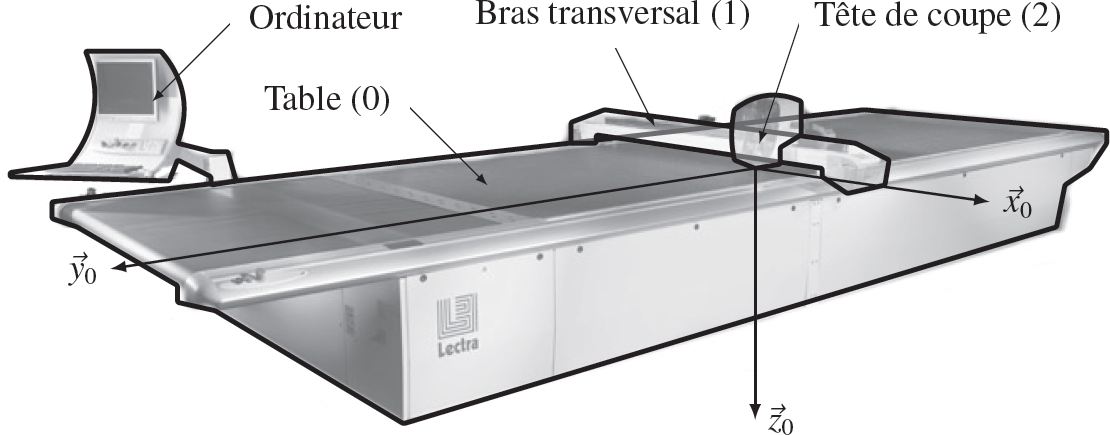
\includegraphics[width=\linewidth]{fig_02}
\end{center}


On donne sur la figure suivant le schéma cinématique spatial d'un des robots avec le paramétrage associé aux différents solides et aux liaisons. 

\begin{center}
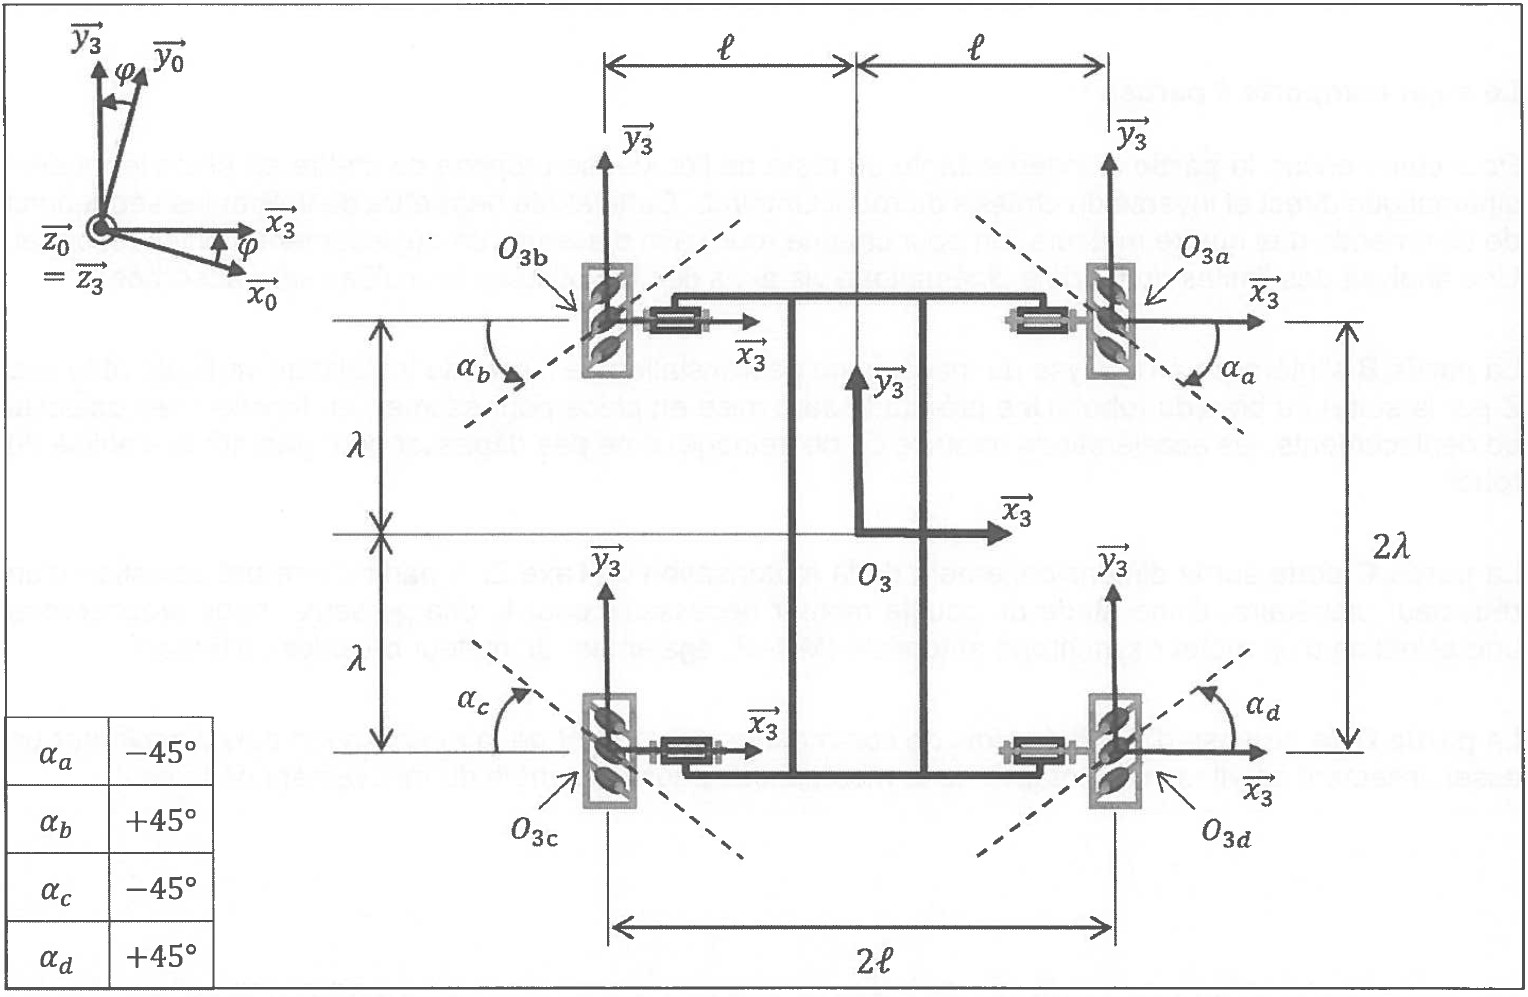
\includegraphics[width=\linewidth]{fig_03}
\end{center}

L'ensemble des repères sont considérés orthonormés directs.


\begin{itemize}
\item On note $\rep{0}=\repere{O_0}{x_0}{y_0}{z_0}$ le repère supposé galiléen associé au sol de la salle de spectacle, appelé bâti \textbf{0}.
\item On note $\rep{1}=\repere{O_0}{x_1}{y_1}{z_1}$ le repère associé à la chaise \textbf{1} et $\theta_1=\angl{x_0}{x_1}=\angl{y_0}{y_1}$ l'angle de rotation de la chaise \textbf{1} par rapport au bâti \textbf{0}.
\item On note $\rep{2}=\repere{A}{x_2}{y_2}{z_2}$ le repère associé à l'épaule \textbf{2}, $\vect{O_0A} = a\vect{z_0} + b\vect{x_1}$ et $\theta_2=\angl{x_1}{x_2}=\angl{z_1}{z_2}$ l'angle de rotation de l'épaule \textbf{2} par rapport à la chaise~\textbf{1}.
\item On note $\rep{3}=\repere{B}{x_3}{y_3}{z_3}$ le repère associé à l'avant-bras \textbf{3}, $\vect{AB} = c\vect{x_2}$ et $\theta_3=\angl{x_2}{x_3}=\angl{z_2}{z_3}$ l'angle de rotation de l'avant-bras \textbf{3} par rapport à l'épaule \textbf{2}.
\item On note $\rep{4}=\repere{C}{x_4}{y_4}{z_4}$ le repère associé au bras \textbf{4}, $\vect{BC} = d\vect{x_3}$ et $\theta_4=\angl{x_3}{x_4}=\angl{y_3}{y_4}$ l'angle de rotation du bras \textbf{4} par rapport à l'avant-bras \textbf{3}.
\item On note $\rep{5}=\repere{D}{x_5}{y_5}{z_5}$ le repère associé à la nacelle \textbf{5}, $\vect{CD} = e\vect{x_4}$ et $\theta_5=\angl{y_4}{y_5}=\angl{z_4}{z_5}$ l'angle de rotation de la nacelle \textbf{5} par rapport au bras \textbf{4}.
\end{itemize}
Le centre de gravité de la nacelle \textbf{5} (siège + volontaire + harnais) est tel que $\vect{DG}=f\vect{x_4}+h\vect{z_5}$. 

On définit la position du point $G$ dans la base $\mathcal{B}_0 = \base{x_0}{y_0}{z_0}$ telle que $\vect{O_0 G} = x\vect{x_0}+y\vect{y_0}+z\vect{z_0}$.
 
\question{Tracer les figures planes de changement de repère.}
\ifprof
\begin{corrige}
\end{corrige}
\else\fi


\question{Exprimer la position du point $G$ suivant $\vect{x_0}$.}
\ifprof
\begin{corrige}
\end{corrige}
\else\fi

\begin{obj}
Valider que l'exigence d'accélération est satisfaite : l'accélération ressentie doit être au maximum de \SI{3,5}{g}.
\end{obj}


%L'accélération ressentie par les volontaires, notée $\vect{\Gamma}_G}=\vecta{G}{5}{0}$ avec $\vect{g}=-g\vect{z_0}$.
%On limite l'étude dans un premier temps au cas où $\theta_1 = \text{cte}$ et donc $\dot{\theta}_1=0$. 


\ifprof
\else
\begin{marginfigure}
\centering

\includegraphics[width=3cm]{Cy_12_Ch_03_Application_03_DanseRobots_qr}
\end{marginfigure}
\fi

\question{Exprimer la vitesse du point $G$ dans son mouvement par rapport au repère galiléen associé à \textbf{0}, notée $\vectv{G}{5}{0}$.}
\ifprof
\begin{corrige}
\end{corrige}
\else\fi

On limite désormais l'étude dans au cas où $\dot{\theta}_2 = \SI{1,45}{rad.s^{-1}}$, ${\theta}_3={\theta}_4={\theta}_5=0$.


\question{Exprimer l’accélération du point $G$ dans son mouvement par rapport au repère galiléen associé à 0, notée $\vectg{G}{5}{0}$.}
\ifprof
\begin{corrige}
\end{corrige}
\else\fi


\question{Conclure quant au respect de l'exigence d'accélération ressentie. }
\ifprof
\begin{corrige}
\end{corrige}
\else\fi


